%#BIBTEX pbibtex paper_jsai2021
%%\documentstyle[twocolumn,jsaiac]{jarticle}
%%\documentstyle[twocolumn,jsaiac]{j-article}
\documentclass[twocolumn]{jarticle}

\usepackage{jsaiac}
\usepackage [dvipdfmx]{graphicx}

\usepackage{listings}
\usepackage{plistings}
\def\lstlistingname{コード}

\usepackage{url}
\newcommand{\bhline}{\noalign{\hrule height 1.5pt}}  % 表のための太いライン

%%% For ASP
\newcommand{\asap}{\textit{teaspoon}}
\newcommand{\gringo}{\textit{gringo}}
\newcommand{\clingo}{\textit{clingo}}
\newcommand{\clasp}{\textit{clasp}}
\newcommand{\asprin}{\textit{asprin}}
\newcommand{\dlv}{\textit{DLV}}
\newcommand{\wasp}{\textit{WASP}}
\newcommand{\code}[1]{\lstinline[basicstyle=\ttfamily]{#1}}
\newcommand{\naf}[1]{\ensuremath{{\sim\!\!{#1}}}}
\newcommand{\head}[1]{\ensuremath{\mathit{head}(#1)}}
\newcommand{\body}[1]{\ensuremath{\mathit{body}(#1)}}
%\newcommand{\atom}[1]{\ensuremath{\mathit{atom}(#1)}}
\newcommand{\poslits}[1]{\ensuremath{{#1}^+}}
\newcommand{\neglits}[1]{\ensuremath{{#1}^-}}
\newcommand{\pbody}[1]{\poslits{\body{#1}}}
\newcommand{\nbody}[1]{\neglits{\body{#1}}}
%\newcommand{\Cn}[1]{\ensuremath{\mathit{Cn}(#1)}}
\newcommand{\reduct}[2]{\ensuremath{#1^{#2}}}

\usepackage{color}

%%
\title{
\jtitle{解集合プログラミングを用いた多目的車両装備仕様問題の解法}
\etitle{Solving Multi-objective Vehicle Equipment Specification
 Problem with Answer Set Programming}
}
%%英文は以下を使用
%\title{Style file for manuscripts of JSAI 20XX}

\jaddress{竹内頼人 \texttt{takeuchi.raito@nagoya-u.jp}}

\author{%
\jname{竹内 頼人\first}
\ename{Raito Takeuchi}
\and
\jname{田村 直之\second}
\ename{Naoyuki Tamura}
\and
\jname{番原 睦則\first}
\ename{Mutsunori Banbara}
%\and
%Given-name Surname\third{}%%英文は左を使用
}

\affiliate{
\jname{\first{}名古屋大学 大学院情報学研究科}
\ename{Graduate School of Informatics, Nagoya University}
\and
\jname{\second{}神戸大学 情報基盤センター}
\ename{Information Science and Technology Center, Kobe University}
%\and
%\third{}Affiliation \#3 in English%%英文は左を使用
}

%%
%\Vol{28}        %% <-- 28th(変更しないでください)
%\session{0A0-00}%% <-- 講演ID(必須)

\begin{abstract}
Answer Set Programming (ASP) is an approach to declarative problem
solving, combining a rich yet simple modeling language with high
performance solving capacities. We here develop an ASP-based approach
to Multi-Objective Vehicle Equipment Specification Problem (MO-VESP).
%
The resulting system reads a MO-VESP instance of OVM format and
converts it into a set of ASP facts. In turn, these facts are combined
with a first-order encoding for MO-VESP solving, which can
subsequently be solved by the ASP solver {\asprin}.
%
In our experiments,
we succeeded in enumerating all Pareto optimal solutions for a
small-scale problem.
\end{abstract}

%\setcounter{page}{1}
\def\Style{``jsaiac.sty''}
\def\BibTeX{{\rm B\kern-.05em{\sc i\kern-.025em b}\kern-.08em%
 T\kern-.1667em\lower.7ex\hbox{E}\kern-.125emX}}
\def\JBibTeX{\leavevmode\lower .6ex\hbox{J}\kern-0.15em\BibTeX}
\def\LaTeXe{\LaTeX\kern.15em2$_{\textstyle\varepsilon}$}

\begin{document}
\maketitle

%%% Local Variables:
%%% mode: latex
%%% TeX-master: "paper"
%%% End:

% LocalWords:  VESP OVM

\section{はじめに}\label{sec:introduction}
% ------------------------------------------
  \thicklines
  \setlength{\unitlength}{1.28pt}
  \small
  \begin{picture}(280,57)(4,-10)
    \put(  0, 20){\dashbox(50,24){\shortstack{根付き全域森\\問題}}}
    \put( 60, 20){\framebox(50,24){変換器}}
    \put(120, 20){\dashbox(50,24){\shortstack{ASPファクト}}}
    \put(120,-10){\alert{\bf\dashbox(50,24){\scriptsize{\shortstack{ASP符号化\\(論理プログラム)}}}}}
    \put(180, 20){\framebox(50,24){ASPシステム}}
    \put(240, 20){\dashbox(50,24){\shortstack{根付き全域森\\問題の解}}}
    \put( 50, 32){\vector(1,0){10}}
    \put(110, 32){\vector(1,0){10}}
    \put(170, 32){\vector(1,0){10}}
    \put(230, 32){\vector(1,0){10}}
    \put(170, +2){\line(1,0){4}}
    \put(174, +2){\line(0,1){30}}
  \end{picture}  

% ------------------------------------------

車両装備仕様とは,簡単に言うと,自動車のカタログに記載されているモデ
ル/グレードと装備の組合せのことである.
車両装備仕様を決めるには,販売される国や地域の法規や規制,
地域や市場の特性,市場の嗜好や競合など十分に考慮する必要があり,
現状では専門知識をもつ技術者の多大な労力が費やされている.
そのため,車両装備仕様探索の自動化・効率化は自動車メーカーにとって
重要な課題の一つである.

\textbf{多目的車両装備仕様問題}は組合せ最適化問題の一種であり,主に装備タイ
プと装備オプションから構成される.
\textbf{装備タイプ}はエンジンやトランスミッションなどの装備の種類を表す.
\textbf{装備オプション}は4気筒エンジン,CVTなどの具体的な装備を表す.
多目的車両装備仕様問題の目的は,
与えられた装備仕様の個数,
装備タイプの集合,
装備オプションの集合から,
装備および燃費に関する制約を満たしつつ,
予想販売台数の最大化や装備オプション数の最小化など,トレードオフの関係にある
複数の目的関数のもとで最適な車両装備仕様を求めることである.

本研究では,燃費に関する制約として,欧米で採用され日本でも2020年度から
導入されている\textbf{企業平均燃費}
(Corporate Average Fuel Efficiency; CAFE~\cite{metimlit18:cafe})
方式を用いる.
このCAFE方式は自動車の燃費規制で,車種別ではなくメーカー全体での出荷台
数を加味した平均燃費を算出し,規制をかける方式である.
CAFE方式の特長は,ある特定の車種では燃費基準を達成できなくても,他の車
種の燃費を向上させることで基準を達成できることが可能な点である.
本論文では,CAFE方式に基づく多目的車両装備仕様問題(以降,\textbf{多目的CAFE問題}と
呼ぶ)を対象とする.

\textbf{解集合プログラミング}
(Answer Set Programming; ASP~\cite{%
  Baral03:cambridge,%
  Gelfond88:iclp,%
  Inoue08:jssst})
は,論理プログラミングから派生した宣言的プログラミングパラダイムである.
ASP言語は一階論理に基づく知識表現言語の一種である.
論理プログラムはASPのルールの有限集合である.
ASPシステムは論理プログラムから安定モデル意味論~\cite{Gelfond88:iclp}
に基づく解集合を計算するシステムである.
近年,SATソルバー技術を応用した高速ASPシステムが実現され,
ロボット工学,システム生物学,システム検証,制約充足問題,プランニング
など様々な分野への実用的応用が急速に拡大している~\cite{Gelfond16:aim}.


提案手法の有効性を評価するために,企業から提供を受けた小規模・中規模・大規模の
多目的CAFE問題に対して実行実験を行った結果,
小規模な問題では5問中4問で最適解の全列挙をすることができた.
\section{CAFE問題}\label{sec:background}

%-------------------------------------------------------
\begin{figure*}[t]
  \centering
  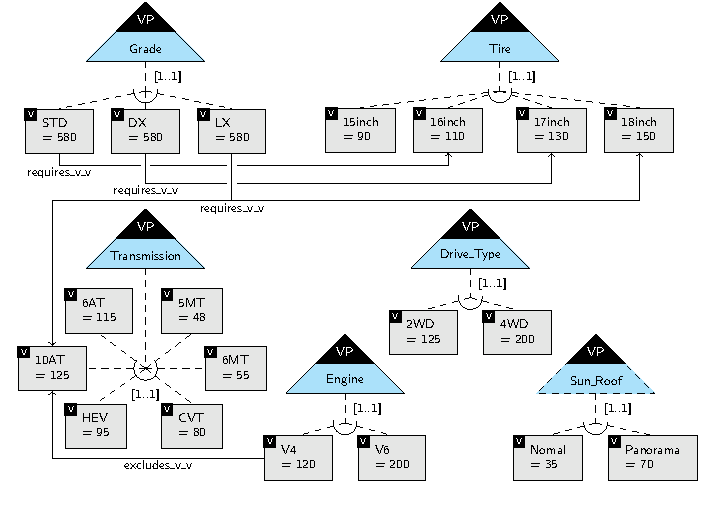
\includegraphics[width=0.8\linewidth]{images/ovm_example.pdf}
  \caption{CAFE問題の例}
  \label{fig:ovm_example}
\end{figure*}
%-------------------------------------------------------

CAFE問題の入力は以下の通りである.
以降,
装備タイプをタイプ,
装備オプションをオプション
と簡単に書くことにする.
\begin{enumerate}
\item タイプの集合\label{input:vp}
\item オプションの集合\label{input:v}
\item タイプとオプションの対応関係\label{input:vp-v}
\item 各タイプで選択可能なオプション数の上下限値\label{input:ublb}
\item タイプ同士,オプション同士,および,タイプとオプション間の依存関係
  \label{input:dependency}
\item 各オプションに付加された IWR 値\label{input:iwr}
%%%
\item 求めたい装備仕様の個数\label{input:g}
\item 各装備仕様とタイプ(あるいはオプション)間の依存関係\label{input:init}
\item 各装備仕様に含まれるオプションの IWR 値の総和と燃費との対応表\label{input:fe}
\item 各装備仕様に含まれるオプションの IWR 値の総和と予想販売台数との対応表\label{input:sv}
\item CAFE 基準値\label{input:cafe}
\end{enumerate}
入力~\ref{input:iwr}の IWR は Inertial Working Rating の略で,
直観的には各オプションの重量を表す.
入力~\ref{input:g}の個数は,求めたい派生車両の数と考えるとわかりやすい.
CAFE問題は,上記の入力から,
装備および燃費に関する制約を満たしつつ,
予想販売台数を最大化する車両装備仕様を求める問題である.

CAFE問題の制約は以下の通りである.
\begin{description}
\item[範囲制約]: 各装備仕様について,各タイプで選択されるオプション数は,
  入力~\ref{input:ublb}で与えられた上下限値の範囲内でなければならない.
\item[依存制約]: 各装備仕様について,入力~\ref{input:dependency}で与
  えられた依存関係を満たさなければならない.
  依存制約には,要求制約と排他制約の2つがある.
\item[燃費制約]: 入力~\ref{input:cafe}の CAFE 基準値を$t$,
  入力~\ref{input:g}の装備仕様個数を$n$として,
  以下の CAFE 規制を満たさなければならない.
  \begin{adjustvboxheight}
  \[
    \begin{array}{lcr}
      & & \\
      \displaystyle\frac{\sum_{i=1}^{n} FE_{i}\cdot SV_{i}}{\sum_{i=1}^{n} SV_{i}}
      &
        \geq 
      &
        t \\
      & & 
    \end{array}
  \]
  \end{adjustvboxheight}
  不等式の左辺は$n$個の装備仕様の\textbf{平均燃費}を表している.
  $FE_{i}$と$SV_{i}$は,装備仕様$i$の燃費と予想販売台数を表しており,
  それぞれ,入力~\ref{input:fe}と\ref{input:sv}の対応表を元に計算される.
\item[初期制約]:
  入力~\ref{input:init}で与えられた依存関係を満たさなければならない.
\end{description}

%%%%%%%%%%%%%%%%%%%%%%%%%%%%
%-------------------------------------------------------
\begin{figure}[tb]
  \centering
  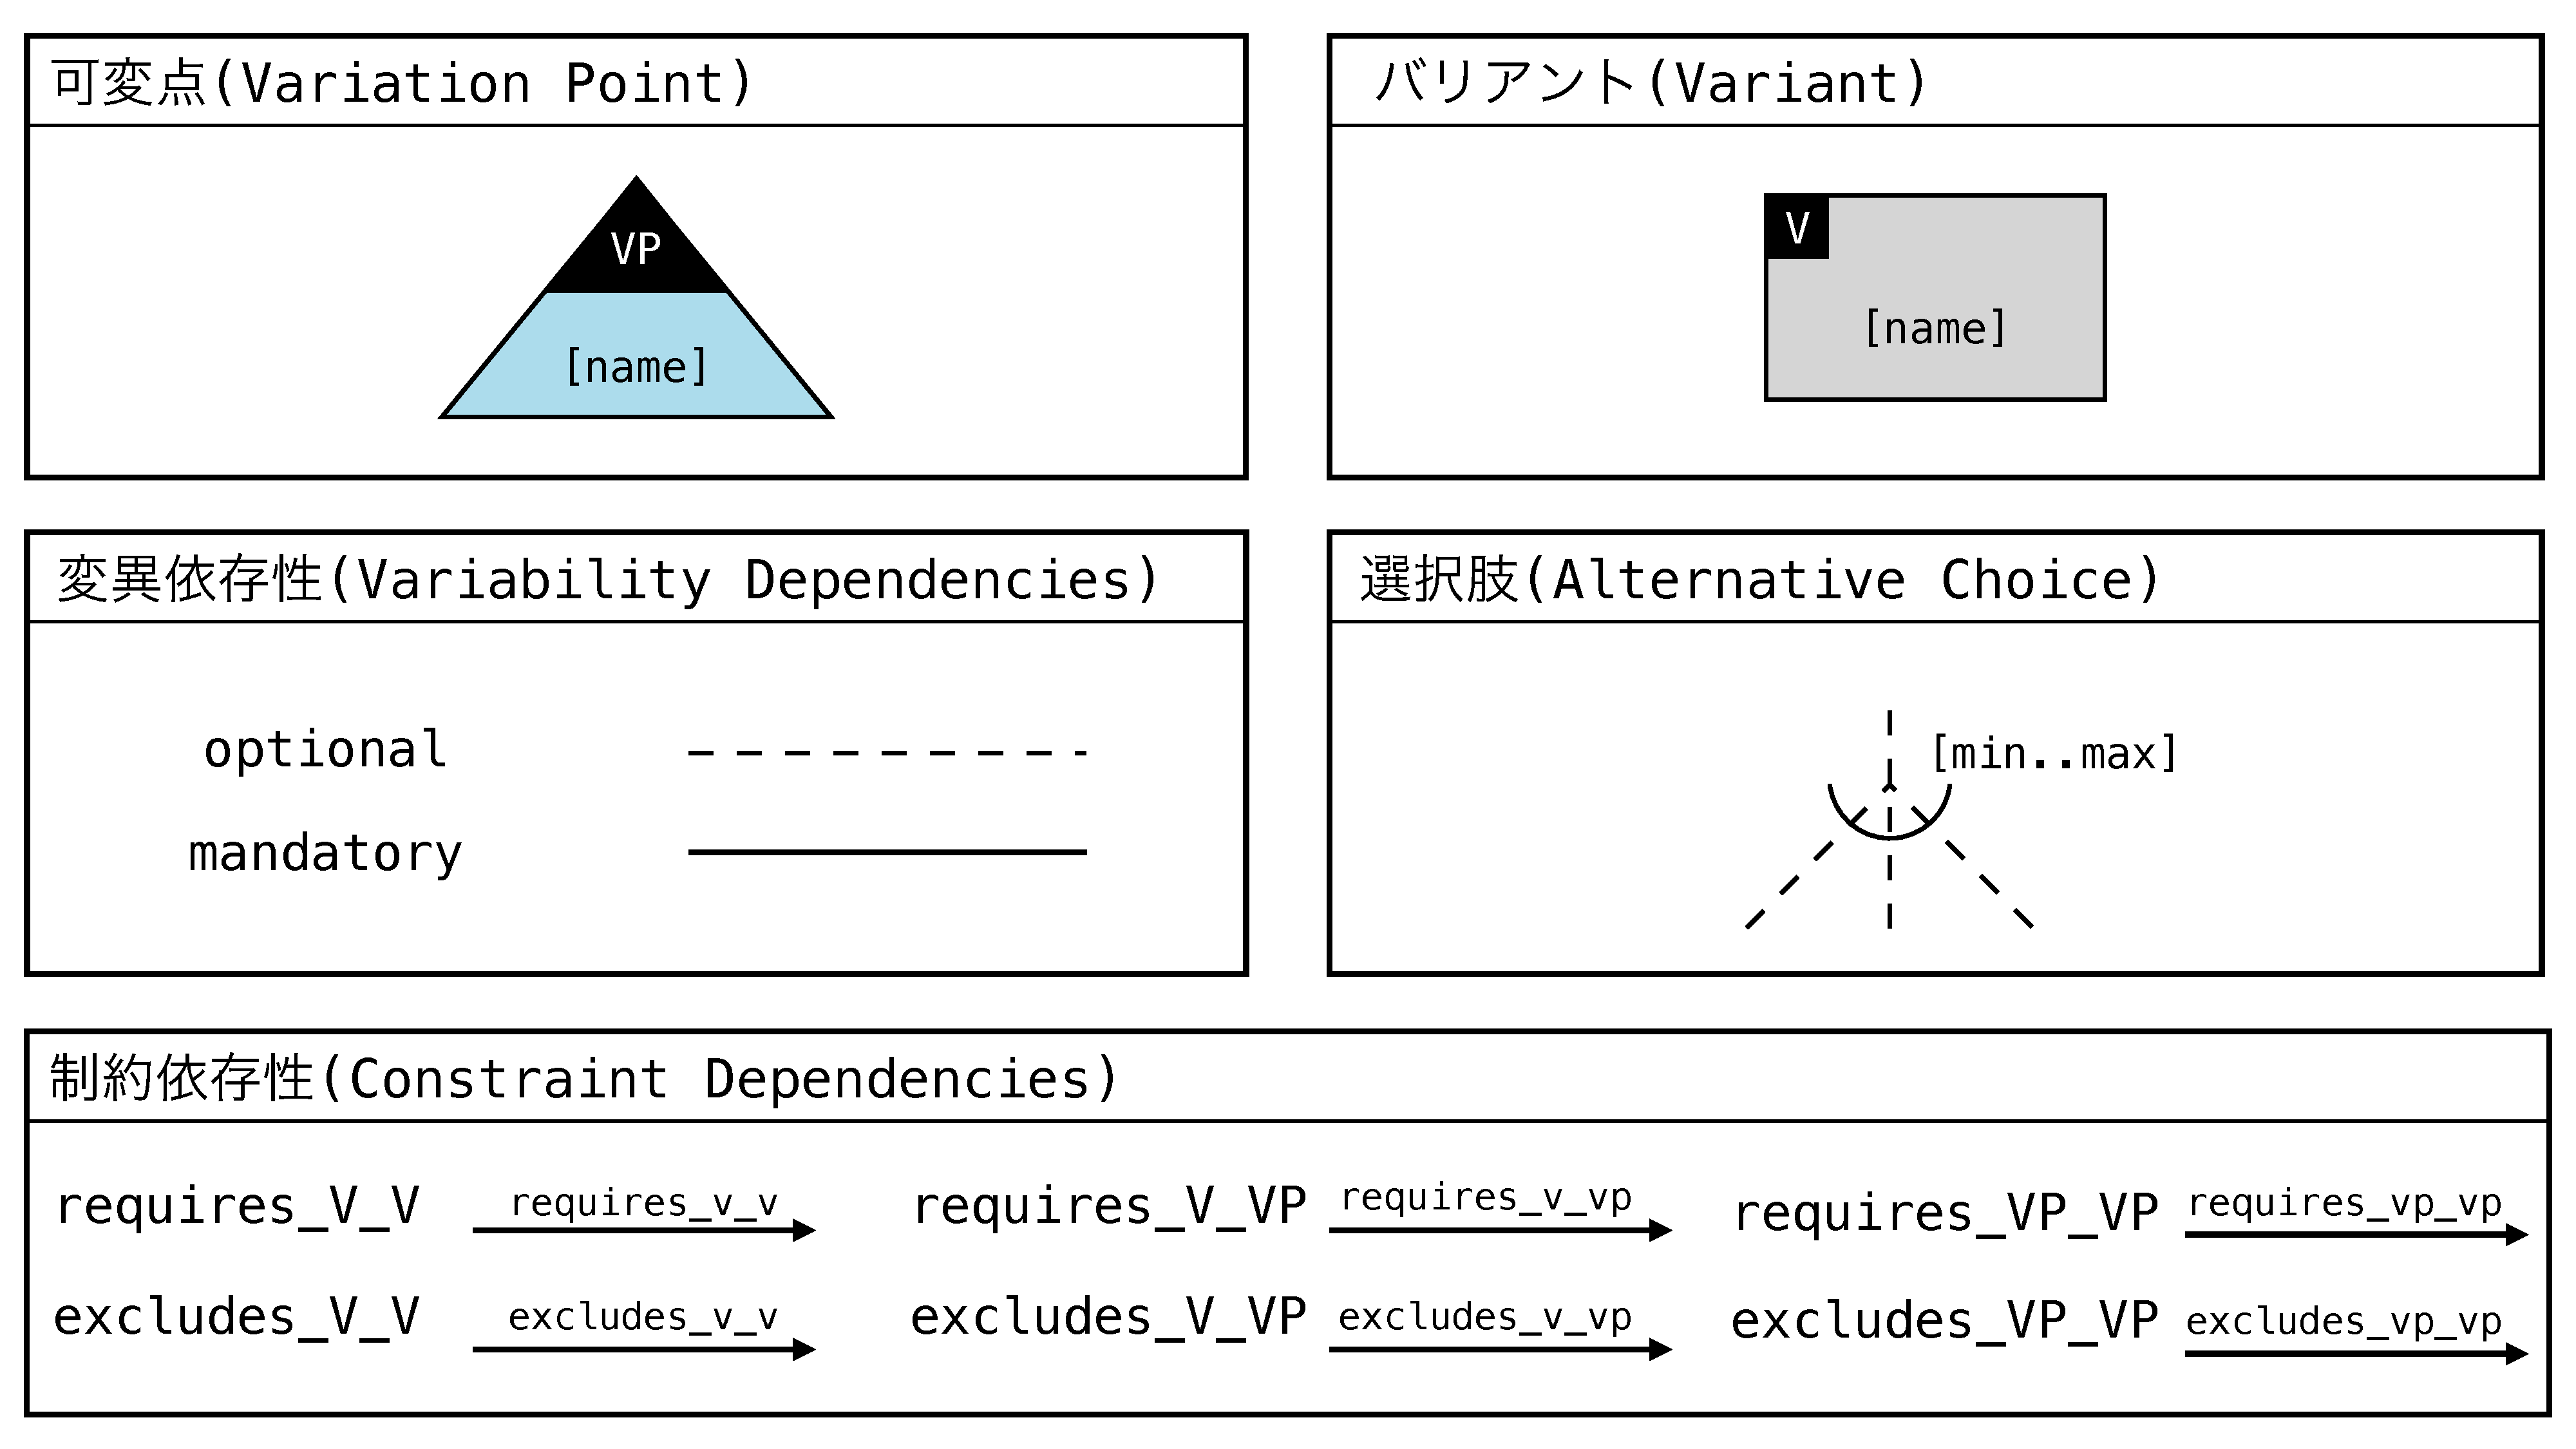
\includegraphics[width=\linewidth]{images/notation.pdf}
  \caption{可変性モデルの表記法\cite{Pohl05:sple}}
  \label{fig:ovm_notation}
\end{figure}
%-------------------------------------------------------

CAFE問題の例を図~\ref{fig:ovm_example}に示す.
この例は,ソフトウェアプロダクトライン開発の分野で用いられる
\textbf{可変性モデル} (Orthogonal Variability Model; OVM\cite{Pohl05:sple})
によって記述されている.
図~\ref{fig:ovm_notation}に,可変性モデルの基本的な表記法を示す.
可変性モデルでは,
仕様ごとに変わりうる項目を\textbf{可変点}と呼び,三角形で表す.
可変点の具体的なインスタンスを\textbf{バリアント}と呼び,長方形で表す.
可変点とバリアントの対応関係には\textbf{変異依存性}と\textbf{選択肢}があり,
選択肢の場合は,その多重度も付記される.
可変点同士,バリアント同士,および,可変点とバリアント間の依存関係は,
\textbf{制約依存性}によって表される.
制約依存性には,要求(\textsf{requires})と排除(\textsf{excludes})の2種類がある.

可変性モデルでCAFE問題を記述する場合,
タイプは可変点,
オプションとその IWR 値はバリアント,
タイプとオプションの対応関係および
選択可能なオプション数の上下限値は選択肢,
タイプ同士,オプション同士,および,タイプとオプション間の依存関係は
制約依存性によって表される.
以上から,CAFE問題の入力のうち,
\ref{input:vp}〜\ref{input:iwr}は可変性モデルによって記述されるこ
とがわかる.

図~\ref{fig:ovm_example}の問題例は,
6個のタイプ,19個のオプション,5個の依存制約から構成され,
各タイプの選択可能なオプション数はすべて1である.
本論文では,可変点で表されるタイプは,各装備仕様に対して必須とする.
ただし,\textsf{Sun\_Roof}のような選択可能なタイプ(必須ではないタイプ)
については,破線の可変点で表すものとする.

%-------------------------------------------------------
\begin{table}[t]
  \centering
  \caption{CAFE問題(図~\ref{fig:ovm_example})の解}
  \begin{tabular}{l|l|c|c|c} \bhline
    %\multicolumn{1}{c|}{装備}   & \multicolumn{3}{c}{装備仕様} \\ \cline{2-4}
    \multicolumn{2}{l|}{装備仕様}               & 1	& 2 	 & 3	\\  \hline
    装備 & \textsf{Grade}        & \textsf{STD}    & \textsf{DX}     & \textsf{LX}\\
    &\textsf{Drive\_Type}  & \textsf{2WD}    & \textsf{2WD}    & \textsf{2WD}\\
    &\textsf{Engine}	  & \textsf{V4}     & \textsf{V6}     & \textsf{V6}\\
    &\textsf{Tire}	  & \textsf{16inch} & \textsf{17inch} & \textsf{18inch}\\
    &\textsf{Transmission} & \textsf{5MT}    & \textsf{6MT}    & \textsf{10AT}\\
    &\textsf{Sun\_Roof}    & -               & \textsf{Normal} & -  \\ \hline
    \multicolumn{2}{l|}{IWR 値の総和}           & 983  & 1,125   & 1,180 \\ %\hline
    \multicolumn{2}{l|}{燃費(km/L)}      & 10.2  & 8.9     & 8.5 \\ %\hline
    \multicolumn{2}{l|}{予想販売台数}    & 745   & 1,988   & 1,171  \\ \hline
    \multicolumn{2}{l|}{平均燃費(km/L)}  & \multicolumn{3}{c}{9.0} \\ 
    \multicolumn{2}{l|}{予想販売台数(合計)}  & \multicolumn{3}{c}{3,904} \\ \hline
 \end{tabular}
 \label{tab:ovm_ans}
\end{table}
%-------------------------------------------------------

図~\ref{fig:ovm_example}の問題に対する解の例を表\ref{tab:ovm_ans}に示す.
この解は,
CAFE 基準値に9.0km/L,
求めたい装備仕様の個数に3を与え,
装備仕様とオプションの依存関係として,
(装備仕様1, \textsf{STD}),
(装備仕様2, \textsf{DX}),
(装備仕様3, \textsf{LX})
を要求して得られたものである.
各装備仕様の燃費(km/L)は,左から順に 10.2, 8.9, 8.5 と
個々には CAFE 基準値を満たしていないが,
3台の平均燃費は 9.028km/L となり,CAFE 規制を満たしている.


%%% Local Variables:
%%% mode: japanese-latex
%%% TeX-master: "paper"
%%% End:

\section{ASPに基づく多目的CAFE問題ソルバー}\label{sec:proposal}

%----------------------------------------
\lstinputlisting[float=t,caption={%
多目的 CAFE 問題(図~\ref{fig:ovm})のASPファクト表現 (車種数$n=3$)},%
captionpos=b,frame=single,label=code:ovm.lp,%
numbers=none,%
breaklines=true,%
columns=fullflexible,keepspaces=true,%
xrightmargin=1zw,% 
xleftmargin=1zw,% 
basicstyle=\ttfamily\scriptsize]{codes/ovm.lp} 
%----------------------------------------

%----------------------------------------
\lstinputlisting[float=tb,caption={%
  多目的 CAFE 問題の ASP 符号化},%
captionpos=b,frame=single,label=code:basic.lp,%
numbers=left,%
breaklines=true,%
columns=fullflexible,keepspaces=true,%
xrightmargin=1zw,% 
xleftmargin=1zw,% 
basicstyle=\ttfamily\scriptsize]{codes/basic.lp} 
%----------------------------------------

提案ソルバーは,可変性モデルで表現された問題インスタンスを ASP のファ
クト形式に変換した後,それらファクトと多目的 CAFE 問題を解くための ASP
符号化と結合し,ASP システム
{\asprin}\footnote{\url{https://potassco.org/asprin/}}
を用いてパレート最適解を求める(図~\ref{fig:arch}参照).
本節では,ASP ファクト形式と ASP 符号化について述べる.
なお,説明の簡単化のため,各装備タイプが選択可能な
装備オプション数の上下限値を1とする.

%%%%%%%%%%%%%%%%%%%%%%%%%%%%%%%%%%%%
\textbf{ASP ファクト形式.}
コード~\ref{code:ovm.lp}は,
CAFE 問題(図~\ref{fig:ovm})を ASP のファクトで表したものである.
%
アトム\code{vp_def/1}は装備タイプ,
\code{v_def/3}は装備オプション,
\code{require_v_v/2}は依存制約(要求),
\code{exclude_v_v/2}は依存制約(排他)
を表している.
例えば,装備タイプ\code{Engine}は,
アトム\code{vp_def("Engine")}で,
その装備オプション\code{V4}は,
アトム\code{v_def("V4", "Engine", 120)}
で表されている.
この他,
\code{require_vp/1}は必須タイプ,
\code{group/1}は車種の識別子を表している.

%%%%%%%%%%%%%%%%%%%%%%%%%%%%%%%%%%%%
\textbf{制約の ASP 符号化.}
多目的 CAFE 問題の ASP 符号化をコード\ref{code:basic.lp}に示す.
%
1行目のルールは,
各車種\code{G},各装備タイプ\code{VP}に対して,
\code{G}が\code{VP}を装備することを意味する
アトム\code{vp(VP,G)}を,ASP の選択肢を用いて導入している.
%
2行目のルールは,各車種\code{G}に対して,
\code{VP}が必須タイプならば,
\code{vp(VP,G)}が成り立たなければならないという制約を表す.
%
5行目のルールは範囲制約を表す.
アトム\code{v(V,G)}は,車種\code{G}が装備オプション\code{V}
を実装することを意味する.
このルールは,車種\code{G}が装備タイプ\code{VP}を装備するならば,
\code{G}は\code{VP}の装備オプションからちょうど1個を選択する制約を表す.
%
16行目のルールは燃費制約を表す.
このルールは,
CAFE 規制の式を以下のように変形し,ASPの重み付き個数制約で表している.
\begin{center}
\(\sum_{g=1}^{n} (FE_{g}-t)\cdot SV_{g} \geq 0\)  
\end{center}
ルール中の定数\code{t}は CAFE 基準値を表し,
{\asprin}の実行時のオプションによって与えられる.
\code{fe(FE,G)}と\code{sv(SV,G)}は,それぞれ,
$FE_{g}$と$SV_{g}$に対応している.
%
19〜22行目のルールは,依存制約(要求)を表す.
例えば,19行目のルールは,
装備オプション\code{V1}と\code{V2}の間に要求的な依存関係があり,
車種\code{G}が\code{V1}を実装するならば,
\code{G}は\code{V2}を実装しなければならない制約を表す.
同様にして,依存制約(排他)も一貫性制約を用いて簡潔に表される.

%%%%%%%%%%%%%%%%%%%%%%%%%%%%%%%%%%%%
\textbf{目的関数の ASP 符号化.}
{\asprin}言語は,解集合の間の選好順序や多目的最適化を記述できるように
拡張されている.
解集合の間の選好順序は,以下の\code{#preference}文によって定義される.
\begin{center}
  \code{#preference(}$s,t$\code{)\{}$e_1,\dots,e_n$\code{\}.}
\end{center}
ここで,$s$は選好名称,$t$は選好タイプ,$e_j$は要素を表す.
{\asprin} では,新たに選好タイプを定義することも可能だが,
\code{subset}, 
\code{less(weight)},
\code{more(weight)},
\code{pareto}
などいくつかの選好タイプはあらかじめ用意されている.
あとは,以下の\code{#optimize}文によって,
選好順序\code{s}について最適な解集合を得ることができる.
\begin{center}
  \code{#optimize(}$s$\code{).}
\end{center}

コード\ref{code:basic.lp}の31行目の\code{#preference}文は,
予想販売台数の最大化を\code{max_sv}という名称で定義している.
同様にして,35行目では,装備オプション数の最小化を
\code{min_op}という名称で定義している.
要素の\code{used_v(V)}は,
装備オプション\code{V}がいずれかの車種において実装されたことを意味する
補助アトムである.
続いて,38行目の\code{#preference}文は,
\code{max_sv}と\code{min_op}の2目的のパレート最適化を
\code{all}という名称で定義している.
最後に,41行目の\code{#optimize}文の要素に\code{all}を与えることによっ
て,多目的 CAFE 問題のパレート最適解を得る.

図~\ref{tab:prt_ans}に,
問題インスタンス (図~\ref{fig:ovm}),
車種数$n=3$,
CAFE 基準値$t=8.5$に対して,
パレート最適解を全列挙をした結果を示す.
解は全部で4つあり,
予想販売台数は右から左へ大きくなり,
装備オプション数は左から右へ小さくなっていることがわかる.

以上のように,ASP に基づく CAFE 問題ソルバーでは,
ASP 言語の表現力の高さを活かし,
多目的 CAFE 問題の制約と目的関数を簡潔に表現できる.
特に,\code{#preference}文を利用することにより,
複数の目的関数を定義・組合せ,柔軟な最適化が可能な点が大きな特長である.

%----------------------------------------

  

\begin{figure*}[t]\centering
  \tabcolsep=1mm
  \begin{tabular}{l|c|c|c||c|c|c||c|c|c||c|c|c}\bhline
    & \multicolumn{3}{c||}{解1} & \multicolumn{3}{c||}{解2} & \multicolumn{3}{c||}{解3} & \multicolumn{3}{c}{解4}\\ \hline
    車種 & 1 & 2 & 3 & 1 & 2 & 3 & 1 & 2 & 3 & 1 & 2 & 3 \\ \hline
    \textsf{Grade} & \textsf{STD} & \textsf{DX} & \textsf{LX} & \textsf{STD} & \textsf{DX} & \textsf{LX} & \textsf{STD} & \textsf{DX} & \textsf{LX} & \textsf{STD} & \textsf{DX} & \textsf{LX} \\
    \textsf{Drive\_Type} & \textsf{2WD} & \textsf{2WD} & \textsf{4WD} & \textsf{2WD} & \textsf{2WD} & \textsf{4WD} & \textsf{2WD} & \textsf{2WD} & \textsf{2WD} & \textsf{2WD} & \textsf{2WD} & \textsf{2WD} \\
    \textsf{Engine} & \textsf{V6} & \textsf{V6} & \textsf{V6} & \textsf{V6} & \textsf{V6} & \textsf{V6} & \textsf{V6} & \textsf{V6} & \textsf{V6} & \textsf{V6} & \textsf{V6} & \textsf{V6} \\
    \textsf{Tire} & \textsf{16inch} & \textsf{17inch} & \textsf{18inch} & \textsf{16inch} & \textsf{17inch} & \textsf{18inch} & \textsf{16inch} & \textsf{17inch} & \textsf{18inch} & \textsf{16inch} & \textsf{17inch} & \textsf{18inch} \\
    \textsf{Transmission} & \textsf{6AT} & \textsf{HEV} & \textsf{10AT} & \textsf{10AT} & \textsf{HEV} & \textsf{10AT} & \textsf{10AT} & \textsf{HEV} & \textsf{10AT} & \textsf{10AT} & \textsf{10AT} & \textsf{10AT} \\
    \textsf{Sun\_Roof} & \textsf{-} & \textsf{-} & \textsf{-} & \textsf{-} & \textsf{-} & \textsf{-} & \textsf{-} & \textsf{-} & \textsf{-} & \textsf{-} & \textsf{-} & \textsf{-} \\\bhline
    予想販売台数(合計)  & \multicolumn{3}{c||}{5,525} & \multicolumn{3}{c||}{5,475} & \multicolumn{3}{c||}{5,135} & \multicolumn{3}{c}{4,723} \\ 
   装備オプション数 & \multicolumn{3}{c||}{12} & \multicolumn{3}{c||}{11} & \multicolumn{3}{c||}{10} & \multicolumn{3}{c}{9} \\ \hline
  \end{tabular}
  \label{tab:prt_ans}
  \caption{多目的 CAFE 問題(図~\ref{fig:ovm})のパレート最適解全列挙}
\end{figure*}


%----------------------------------------
%%% Local Variables:
%%% mode: japanese-latex
%%% TeX-master: "paper"
%%% End:

\section{実行実験}
%----------------------------------------------
\begin{table}[t]\centering
  \caption{ベンチマーク問題}
  \vskip 1em
  % \renewcommand{\arraystretch}{0.9}
  % \tabcolsep = 0.9mm
  \begin{tabular}{lrrrr}\hline
    問題名 & \#装備タイプ	& \#装備オプション	& \#依存制約 	\\\hline
    small   & 8		& 21	& 4	  	        \\
    medium  & 86	& 229	& 147	  	        \\
    big	    & 315	& 1,337	& 0	          	\\\hline
    & & & \\
  \end{tabular}
 \label{tab:bench}
\end{table}
%----------------------------------------------

%----------------------------------------------
\begin{table}[t]\centering
  \caption{実験結果: CPU時間}
  \vskip 1em  
  % \renewcommand{\arraystretch}{0.9}
  % \tabcolsep = 0.9mm
  \begin{tabular}{cr|rr}\hline
    \lw{問題名} & CAFE & パレート   & \lw{CPU時間(秒)} \\
           & 基準値$t$ & 最適解の数 &  \\ \hline
    small  & 8.5   & 8*      &   35.136     \\
    small  & 9.0   & 5*      & 1085.354     \\
    small  & 9.5   & --       & $timeout$    \\
    small  & 10.0  & 1*      &    1.863     \\
    small  & 10.5  & 0*      &    0.221     \\\hline
  \end{tabular}
  \label{tab:result}
\end{table}
%----------------------------------------------

提案ソルバーの有効性を評価するために,多目的 CAFE 問題のパレート
最適解を全列挙する実行実験を行った.
ベンチマーク問題には,企業から提供を受けた3問を使用した(表~\ref{tab:bench}参照).
small は小規模な問題,
medium は現実規模の問題,
big は大規模な問題である.
各問題に対して,
5種類の CAFE 基準値$t = 8.5, 9.0, 9.5, 10.0, 10.5$km/Lを適用し,
計15問に対して実験を行なった.車種の数は$n=3$とした.
ASPシステムには{\asprin}-3.1.1を利用し,
1問あたりの制限時間は3時間とした.
実験環境は,Mac OS, 3.2GHz Intel Core i7, 64GB メモリである.

表~\ref{tab:result}に小規模な問題smallの実験結果を示す.
左の列から順に,問題名,CAFE基準値$t$,得られたパレート最適解の数,
解の全列挙に要した CPU 時間となっている.
記号`$\ast$'は,パレート最適解の全列挙に成功したことを意味する.
逆に,記号`--'は,パレート最適解が一つも得られなかったことを意味する.
%
実験の結果,5問中3問に対して,パレート最適解を全列挙することができた.
また,$t=10.5$の場合のパレート最適解の数は0であり,実行可能解が存在し
ないことが確認できた.
medium と big については,実行可能解は得られたものの,パレート最適解を
得ることはできなかった.

%%% Local Variables:
%%% mode: japanese-latex
%%% TeX-master: "paper"
%%% End:

\section{おわりに}

本論文では,ASP に基づく多目的 CAFE 問題ソルバーの実装と評価について述べた.
ASP 言語の表現力の高さを活かし,
多目的 CAFE 問題の制約と目的関数を簡潔に表現できることを確認した.
企業から提供を受けたベンチマーク問題を用いて評価実験を行った結果,
小規模な問題に対して,パレート最適解を全列挙をすることができた.

今後の課題は,実用規模以上の問題インスタンスに対する,
現実的な計算時間によるCAFE問題の解法の実現である.
そのために,実験ログや問題インスタンスの調査をもとに,
計算のボトルネックとなる部分を特定し,より効率的な符号化を考案したい.
さらに,ソルバーの実用性を高めるために,
協力企業から提案を受けている認証制約,適用タイミング制約,
IWRテーブル制約など,CAFE問題に対する様々な追加制約の実装も行いたい.
%%%%%%%%%%%%%%%%%%%%%%%%%%%%%%%%%%%%%%%%%%%%%%%%%%%
\vskip 1em
\begin{itemize}\Large
\item 関連研究(DONE)
\item 参考文献追加(DONE)
\item 今後の課題(DONE)
\end{itemize}
%%%%%%%%%%%%%%%%%%%%%%%%%%%%%%%%%%%%%%%%%%%%%%%%%%%


%%% Local Variables:
%%% mode: latex
%%% TeX-master: "paper"
%%% End:


\bibliographystyle{jsai}
\bibliography{jsai2021}
\end{document}
